\chapter{Generación de modelos predictivos para el auto-escalado de E-SilboPS} \label{chp:modelos}


En este capítulo, se aborda la generación de los modelos predictivos, mediante
la implementación de algoritmos de Machine-Learning y Deep-Learning, que 
usarán los resultados de las pruebas de rendimiento para predecir el 
comportamiento del sistema.

%%%%%%%%%%%%%%%%%%%%%%%%%%%%%%%%%%%%%%%%%%%%%%%%%%%%%%%%%%%%%%%%%%%%%%%%%%%%%%%%
%%%%%%%%%%%%%%%%%%%%%%%%%%%%%%%%%%%%%%%%%%%%%%%%%%%%%%%%%%%%%%%%%%%%%%%%%%%%%%%%

\section{Modelos predictivos} \label{sct:modelos_modelos-pred}
% Explicar los modelos y qué hacen

Además de estos modelos, también se ha implementado la capacidad de calcular
la primera derivada de los resultados de los modelos, pudiendo obtener resultados
más detallados.

\subsection{Métodos de Series Temporales}

Los primeros modelos que se han implementado han sido los de Series Temporales,
que hacen uso de ''Rolling Forecasting Origin''\cite{web:caret} para ajustar dichos
modelos y poder realizar predicciones.

Para comprobar los resultados de estos modelos, se comparan los valores de la
predicción con todos los anteriores, no solo con el inmediatamente anterior, lo
que lleva a un mejor ajuste de estos modelos al aumentar la precisión de dichas 
predicciones.

\subsubsection*{Rolling Forecasting Origin}

Este método permite dividir una serie de datos temporales en dos series de datos,
una de entrenamiento, y otra de pruebas, de forma que los modelos se puedan ajustar 
con la primera, y se prueben con la segunda.

Esta división se lleva a cabo mediante especificar el tamaño inicial de cada serie,
es decir, el número de valores de la serie temporal que se usarán de forma inicial;
y variando el horizonte, que es el número valores consecutivos en la serie de prueba.

De esta forma, y mediante el tamaño inicial, se establecen el número de repeticiones
de este método (''resampling''), aumentando/moviendo las series temporales de 
entrenamiento y pruebas, tal como se ve en la \autoref{fig:models_time-series}.

Adicionalmente, se puede establecer que la serie de entrenamiento añada los nuevos
valores a los anteriores, de forma que esta crezca con cada repetición.

\begin{figure}[htpb]
    \centering
    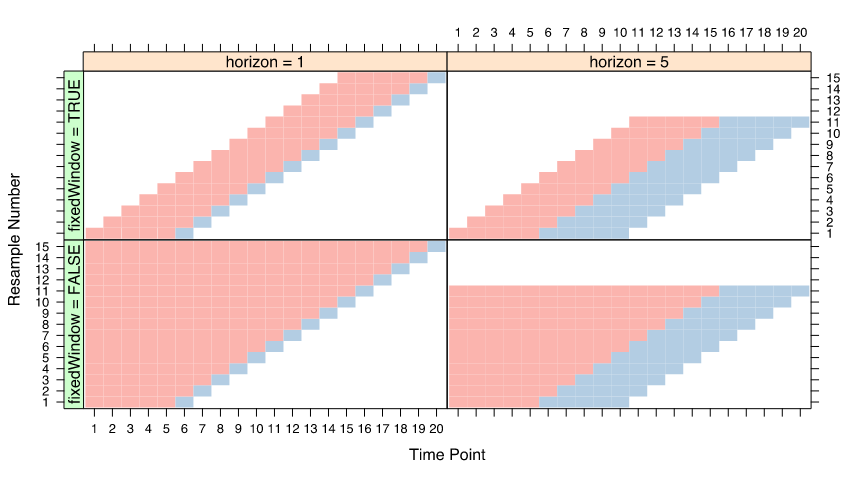
\includegraphics[width=\textwidth]{images/time-series.png}
    \caption{Aplicación de ''Rolling Forecasting Origin'' a una serie de 20 elementos con un tamaño inicial de cada serie de 5 elementos. Los elementos en rojo pertenecen a la serie de entrenamiento, los azules a la serie de pruebas. Imagen obtenida de \cite{web:caret}}
    \label{fig:models_time-series}
\end{figure}

\subsubsection*{Modelos ARIMA}

La implementación del modelo ARIMA, acrónimo del inglés Autoregressive Integrated 
Moving Average, y generalización del modelo ARMA, acrónimo del inglés
Autoregressive Moving Range; permite, mediante el uso de la variación y regresión
de los datos estadísticos, encontrar patrones en dichos datos para poder realizar
predicciones a futuro.

Este proceso se lleva a cabo mediante ajustar el modelo con una serie de datos
de entrenamiento, tras lo que se procede a comprobar si el modelo se ajusta de forma
correcta. Una vez ajustado y comprobado el modelo, este puede generar nuevas
predicciones.

\subsubsection*{Modelos STL con ETS\footnote{https://otexts.com/fpp2/weekly.html}}

También se ha implementado el modelo STL, acrónimo del inglés 
''Seasonal and Trend decomposition using Loess'', para descomponer las 
series temporales junto con el modelo ETS, acrónimo del inglés ''Error, Trend 
and Seasonal''.

Estos modelos obtienen predicciones de los datos ajustados estacionalmente mediante 
aplicar a estos predicciones no estacionales, y reajustando esa estacionalidad
usando los últimos datos de la serie de datos originales (ajustados estacionalmente).

\subsection{Modelos de Machine-Learning y Deep-Learning}

\subsubsection*{Modelos de Regresión Lineal}

Los modelos de Regresión Lineal utilizan las dos variables presentes en los datos,
en este caso, throughput y tiempo, para aproximar la relación de dependencia entre
ambas variables.

Una vez conocida la relación entre ambas variables, el modelo puede predecir futuros
valores en base a dicha relación.

\subsubsection*{Modelos Generalizados Aditivos}

Los Modelos Generalizados Aditivos son una extensión de los Modelos Lineales 
Generalizados, y consideran que la relación entre las variables respuesta (la variable
que queremos predecir, en este caso, el throughput) y las variables explicativas (la
variable que se utiliza para realizar las predicciones, en este caso, el tiempo) puede
tomar cualquier forma funcional, no únicamente lineal.

Mediante esta consideración, estos modelos toman los datos y realizan predicciones
mediante la aplicación de la relación entre ambas variables y las funciones que pueden
representar.

\subsubsection*{Modelos Generalizados Lineales}

Los Modelos Generalizados Lineales generalizan la Regresión Lineal permitiendo que
el modelo lineal se relacione con la variable de respuesta a través de una función
de enlace y permitiendo que la magnitud de la varianza de cada medida sea una función
de su valor predicho.

Esto permite al modelo realizar predicciones mediante aplicar los datos ya obtenidos
y la función de enlace, que depende de la distribución de los propios datos.

\subsubsection*{Modelos de ''Random Forest''}

Los modelos de ''Random Forest'' aplican los datos a un algoritmo de Machine-Learning 
que combina múltiples árboles de decisión clasificando y aplicando regresión a dichos
datos.

Este algoritmo se entrena aprendiendo a clasificar los datos obtenidos, de forma
que el ''random forest'' crece conforme aprende a clasificar nuevos elementos, de 
forma que con nuevos datos no clasificados, sea capaz de predecir su clasificación,
es decir, el algoritmo, una vez entrenado, será capaz de predecir el comportamiento
del sistema al clasificar los nuevos datos recibidos.

\subsubsection*{Modelos de Redes Neuronales}

De forma similar a los modelos de ''Random Forest'', los modelos de redes neuronales
utilizan los datos obtenidos para entrenar una red neuronal que, una vez entrenada,
podrá predecir el comportamiento del sistema mediante clasificar los nuevos valores.\\


De forma adicional, este programa permite aplicar la primera derivada previa aplicación 
de estos modelos predictivos, pudiendo obtener la pendiente de las predicciones 
realizadas.


%%%%%%%%%%%%%%%%%%%%%%%%%%%%%%%%%%%%%%%%%%%%%%%%%%%%%%%%%%%%%%%%%%%%%%%%%%%%%%%%
%%%%%%%%%%%%%%%%%%%%%%%%%%%%%%%%%%%%%%%%%%%%%%%%%%%%%%%%%%%%%%%%%%%%%%%%%%%%%%%%

\section{Resultados esperados} \label{sct:desarrollo_resultadosesperados}

En el momento de la escritura de este Trabajo de Fin de Grado, debido a 
problemas de tiempo, causados por retrasos en el desarrollo de pruebas y 
obtención de resultados previos, no se ha podido aplicar y probar estos
modelos de predicción.

A pesar de esto, al conocer el funcionamiento de estos modelos, se pueden
esperar ciertos resultados de la aplicación de los mismos a este trabajo.

Estos resultados esperados mostrarán una predicción del comportamiento del sistema
en base a los valores anteriores, generando una gráfica en la que se mostrarán
los datos anteriores junto con las predicciones de los modelos, generando un
gráfico similar al de la \autoref{fig:models_results}.

\begin{figure}[htpb]
    \centering
    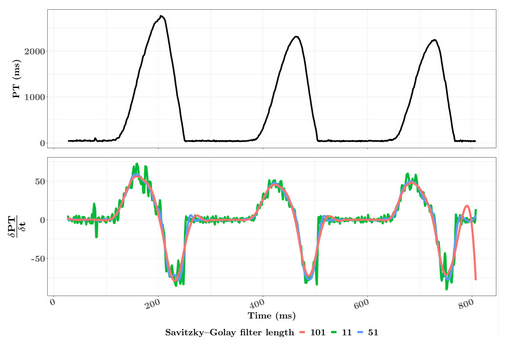
\includegraphics[width=0.5\textwidth]{images/ejemplo-res.png}
    \caption{Ejemplo de resultado de los modelos predictivos.}
    \label{fig:models_results}
\end{figure}